This chapter presents an overview of contributions in the area of engineering \ac{BDI} \ac{MAS} targeting the goal outlined in \ref{rq:5} of making \ac{BDI} \ac{MAS} engineering more accessible for developers wishing to integrate \ac{BDI} agents into larger software systems, there including \acp{DTE} and more broadly Web-based systems.
%
Additionally, the chapter explores the role of \emph{explainability} in \ac{BDI} agents, to make agent behavior more transparent to users, as this is a key requirement for intelligent applications applied to critical domains such as healthcare (\Cref{sec:back:h40:explainable-ai}).

%=======================================================
\section{Tooling for \acs{BDI} Agent Programming}
\label{sec:mas:engineering:jakta}
%=======================================================

\ac{BDI}~\cite{rao1991modeling} agents are considered
an excellent tool for modelling autonomous or intelligent entities
via high-level \emph{cognitive} abstractions.
%
Therefore, in the early 2000s, the expectation of the community was for \ac{AOP}~\cite{Shoham_1993} to gain its spot among other prominent paradigms,
such as object-oriented (\acs{OOP}), functional (\acs{FP}), imperative (\acs{IP}), and logic (\acs{LP}) programming.

However,
a few decades later,
it can be observed that,
although \ac{BDI} has deeply impacted the research field of \ac{MAS} and \ac{AI},
it still fails at reaching mainstream programming,
even in contexts where the application scenario would make it
a good choice to design autonomous behavior.

Limited adoption of \ac{BDI} in mainstream programming has been widely discussed~\cite{lind2000aose,DBLP:journals/sigsoft/MascardiWR19,DBLP:journals/ijaose/DignumD10,DBLP:books/sp/14/Muller014,DBLP:journals/corr/abs-1209-1428}, with no consensus on the root causes.
%
Some argue that improved tooling is needed~\cite{DBLP:conf/dalt/Hindriks14},
while others suggest that the main barrier is the cost of learning a new paradigm~\cite{DBLP:journals/ijaose/Logan18} without the gain of significant benefits in terms of engineering complex behavior, claiming that new features are needed to make \ac{BDI} more appealing.

These perspectives are not necessarily conflicting, but rather arguably complementary: paradigm adoption depends on both effective abstractions and supportive tools.
%
In \cite{DBLP:journals/ijaose/Logan18} \cpp is mentioned as an example of language that despite little tooling support at its inception, gained popularity thanks to the introduction of new abstractions (e.g., classes) that made it more appealing to mainstream developers.
%
It could be argued that it was the seamless, gradual integration of such new abstractions into existing \ac{IP} practices that made \cpp successful.
%
As seen in the evolution of \cpp and Java, such gradual integration of new abstractions can lower adoption barriers and foster community-driven innovation.
%
Thus, paradigm and tooling evolution should proceed in parallel to facilitate broader adoption, possibly by integrating \ac{BDI} concepts into existing mainstream programming practices, paradigms, software ecosystems, and tools.

%-------------------------------------------------------
\subsection{State of the Art}
%-------------------------------------------------------

Several open-source, publicly available, and actively maintained\footnote{Following the definition in~\cite{Cardoso_Ferrando_2021}.} frameworks exist for \ac{BDI} \ac{AOP} programming.
This section highlights representative frameworks, based on recent surveys of logic-based agent-oriented technologies~\cite{lptech4mas-jaamas35} and agent-based programming for \ac{MAS}~\cite{Cardoso_Ferrando_2021}.

\Cref{tab:frameworks} summarizes key characteristic of selected frameworks.
%
Other notable actively developed frameworks that did not meet the selection criteria but still deserve mention are
\jack{}~\cite{Winikoff2005} (not open-source),
the aforementioned \jacamo{}~\cite{Boissier_Bordini_Hübner_Ricci_Santi_2013} frameworks which extends \jason{} (\Cref{sec:back:mas:aose}),
\sarl{}~\cite{iat2014sarl} (not \ac{BDI}-specific),
and \goal{}~\cite{Hindriks2009} (not \ac{BDI}-adhering).

This short overview highlights how existing frameworks differ in terms of intended target applications, execution platforms and agent programming syntax.
%
A more in-depth analysis of the state-of-the-art frameworks is presented in \cite{DBLP:journals/sncs/BaiardiBCP24}, 
focusing on their features and limitations.
%
From this analysis, it is possible to observe that
most frameworks are build with custom \ac{DSL} syntaxes that require learning new languages, as well as dedicated supporting tools (e.g., IDE plugins) that require additional effort to set up and maintain.
%
This also hinders integration with existing software ecosystems and tools, as well as reuse of existing libraries and components, as the mechanisms to interface with external code are often limited and not always straightforward to use, requiring developers to shift their mindset away from familiar programming practices.

\begin{table}
    \centering
    \small
    \resizebox{\textwidth}{!}{
    \begin{tabular}{r|c|c|c}
        \textbf{Framework } & \textbf{Platform} & \textbf{Syntax} & \textbf{Intended Target} \\\hline\hline
        \textbf{\makecell[r]{\astra~\cite{CollierRL15}} }
        & JVM
        & custom DSL
        & distributed systems
        \\
        \textbf{\makecell[r]{\gwendolen~\cite{dennis2008gwendolen}} } 
        & \makecell[c]{MCAPL~\cite{Dennis2018}}
        & \agentspeak{}-based
        & \ac{BDI} verification
        \\
        \textbf{\makecell[r]{\jadex~\cite{PokahrBL2005}} } 
        & JVM
        & Java + annotations
        & distributed systems
        \\
        \textbf{\makecell[r]{\jason~\cite{Bordini_Hübner_Wooldridge_2007}} } 
        & JVM
        & \agentspeak{}
        & \ac{BDI} research
        \\
        \textbf{\makecell[r]{\jsson~\cite{DBLP:conf/emas/KampikN19}} } 
        & JavaScript
        & JavaScript
        & Web applications
        \\
        \textbf{\makecell[r]{\lightjason~\cite{aschermann2016eumas}} } 
        & JVM
        & \agentspeak{}-based
        & scalable applications
        \\
        \textbf{\makecell[r]{\phidias~\cite{DUrsoLS19}} } 
        & (Micro)Python
        & Python DSL
        & IoT/robotic applications
        \\
        \textbf{\makecell[r]{\spadebdi~\cite{PalancaRCJT22}} } 
        & Python
        & \agentspeak{}
        & distributed systems
        \\
        \hline
        \textbf{\makecell[r]{\jakta~\cite{DBLP:journals/sncs/BaiardiBCP24}} } 
        & JVM*
        & Kotlin DSL
        & general-purpose
        \\
    \end{tabular}
    }
    \normalsize
    \bigskip
    \caption{
        A selection of active \ac{BDI} programming frameworks
        and their respective execution platforms, syntax and intended target.
        \jakta{}, the framework proposed in this section, is included to compare with existing frameworks.
        *\jakta{} is currently implemented on the JVM 
        but could be ported to other platforms thanks to Kotlin's multiplatform capabilities.
    }
    \label{tab:frameworks}
\end{table}


%-------------------------------------------------------
\subsection{Desiderata for Mainstream \acs{BDI} Tooling}
%-------------------------------------------------------

As emerging from the previous section,
the \ac{BDI} \ac{AOP} community has primarily developed toolkits
as libraries, extensions, or entirely custom languages
supported by existing execution platforms.
%
This approach provides a practical environment for prototyping and deployment,
allowing developers to leverage the features of the \emph{host} platform.
%
Hence,
a \ac{BDI} framework typically expects users to work in a top-down manner,
approaching system design as a \ac{MAS} and using \ac{BDI} abstractions to model agents,
while leveraging the host language primarily for implementing vertical, low-level, practical details.

Although this may be effective for \ac{BDI} experts
it may pose a barrier for newcomers.
%
An effective way to learn a new paradigm is to start with a simple yet functional fragment,
then incrementally expand its functionalities,
gradually introducing new concepts and abstractions (example-based learning, see~\cite{vanGog2010}).


Based on these considerations and the analysis of existing frameworks, the following desiderata for mainstream \ac{BDI} tooling are identified:

\paragraph{Interoperability with Mainstream Paradigms:} to have \ac{BDI} work as a \emph{practical} paradigm it is necessary to integrate with external systems that typically are not built using \ac{BDI} concepts, which results in a developer to likely incorporate other paradigms in parts of the developed system.
%
Many modern programming languages (including Kotlin, Python, Scala, etc.) are designed to be \emph{multi-paradigm}, allowing developers to switch among paradigms with relative ease.
%
This approach, known as \emph{paradigm blending},
prioritizes integration of multiple paradigms in one code fragment
over composition of multiple fragments using different paradigms.
%
When paradigms are blended,
the same code fragment may contain \emph{syntactical}
constructs capturing abstractions of diverse paradigms.
%
In this context, \ac{BDI} \ac{AOP} could be envisioned
as yet another paradigm to support,
letting developers free to use a mix of different abstractions in the same codebase.


\paragraph{Code Reuse and Sharing Mechanisms:}

Code reuse is fundamental in software engineering for reducing redundancy and improving maintainability. General-purpose languages support reuse through constructs such as packages, modules, classes, and functions, complemented by import and extension mechanisms.
%
This is important for both \emph{in-project} reuse, but especially for \emph{cross-project} reuse, enabling the creation and sharing of libraries and frameworks. These are usually supported by build automation and dependency management tools that facilitate integration and versioning.
%
In \ac{AOP}, similar mechanisms would enable modularization and reuse of agent specifications. For \ac{BDI} \ac{MAS}, this could involve sharing plans, beliefs, or rules across agents. However, there is no standardized approach for modularity and reuse at the paradigm level.
%
When a framework provides a \ac{FFI}, reuse mechanisms from the host language can be applied to relevant code sections. For example, \jason{} and \spadebdi{} allow internal actions to be defined and reused as Java or Python code, respectively.
%
For code written in the \ac{BDI} language, reuse is often limited to file inclusion (e.g., like in \jason{}). Some like \astra{}, support specification extension, while others, such as \jack{} and \jadex{}, use capabilities~\cite{DBLP:conf/promas/BraubachPL05} to encapsulate reusable components, though interpretations vary.


\paragraph{Development Tools:}
Development tools are critical for effective \ac{BDI} programming.
Modern development environments offer features such as syntax highlighting, code completion, static analysis, and refactoring, which are now expected for a swift development experience.
%
Testing libraries and debugging support are also essential for building reliable systems. However, most \ac{BDI} frameworks lag behind mainstream languages in tool maturity, often due to the high maintenance cost for small communities and limited incentives in tool development in research-driven projects.
%
Developing and maintaining compatibility of plugins for target development environments is challenging.
%
This can be alleviated by developing \emph{internal} \acp{DSL} which can directly leverage existing tools, though sometimes at the expense of language expressiveness.
%
Testing and debugging \acp{MAS} remain complex. \ac{BDI} frameworks offer limited support, and recent efforts~\cite{DBLP:conf/atal/RodriguezTW23,amaral2023atal} are still maturing. Additionally, debugging through host language tools is possible but often exposes low-level details irrelevant to \ac{BDI} abstractions.
%
Simulation is another important tool, especially for distributed systems. Existing \ac{MABS} frameworks are not tailored for \ac{BDI} agents, leading to an abstraction gap and duplicated effort when implementing both production and simulation environments. Ideally, frameworks should facilitate seamless switching between real and simulated deployments as discussed in \Cref{sec:mas:engineering:simulation}

\paragraph{Configurability:}
\ac{BDI} frameworks also manage the runtime environment for agents, including input/output, communication, and concurrency models (\Cref{ssec:mas:engineering:concurrency}). Configurability in these aspects is essential for adapting frameworks to diverse application requirements.
%
The concurrency model, mapping the agent control flow to execution primitives (e.g., threads, processes, event loops), directly impacts efficiency, determinism, and reproducibility and affects system performance. Most frameworks support one or more concurrency models, but few offer user-oriented APIs for easily customizing or selecting the concurrency model.
%
Agent communication is another key aspect, with frameworks differing in their support for local and distributed messaging. Communication typically relies on agent communication languages (ACLs)~\cite{Kone_Shimazu_Nakajima_2000} and underlying network protocols.
%
Pluggable communication mechanisms, using standard protocols, are considered good practice, allowing users to select or extend protocols as needed. However, multi-protocol support and well-documented APIs for communication configuration remain uncommon.
%
Overall, high configurability in concurrency and communication is a desirable property for mainstream \ac{BDI} tooling, enabling broader applicability and easier integration with existing systems.

%-------------------------------------------------------
\subsection{The \jakta{} Framework}
%-------------------------------------------------------

\jakta{} is a new \ac{BDI} programming framework,
aimed at (gradually) addressing the issues discussed in the sections above.
%
\jakta{} is available on GitHub\footnote{\url{https://github.com/jakta-bdi/jakta}}
under a free, open-source, and permissive licence.
%
The main design principles of the tool are \emph{modularity},
\emph{pluggability} and
\emph{paradigm interoperability}.

\jakta{} clearly separates:
\begin{inlinelist}
    \item definition of concepts (e.g., agents, environment, plans, actions),
    \item the logic that rules concepts' behavior (e.g., execution loops, selection functions),
    and
    \item how these are presented to the final user (e.g., syntax, \ac{API}).
\end{inlinelist}
%
Multi-paradigm interoperability is obtained by designing \jakta{} as an internal \ac{DSL} in Kotlin,
thus leveraging Kotlin's multi-paradigm features that already support \ac{OOP}, \ac{FP}, and \ac{IP} styles.

\begin{figure}
    \centering
    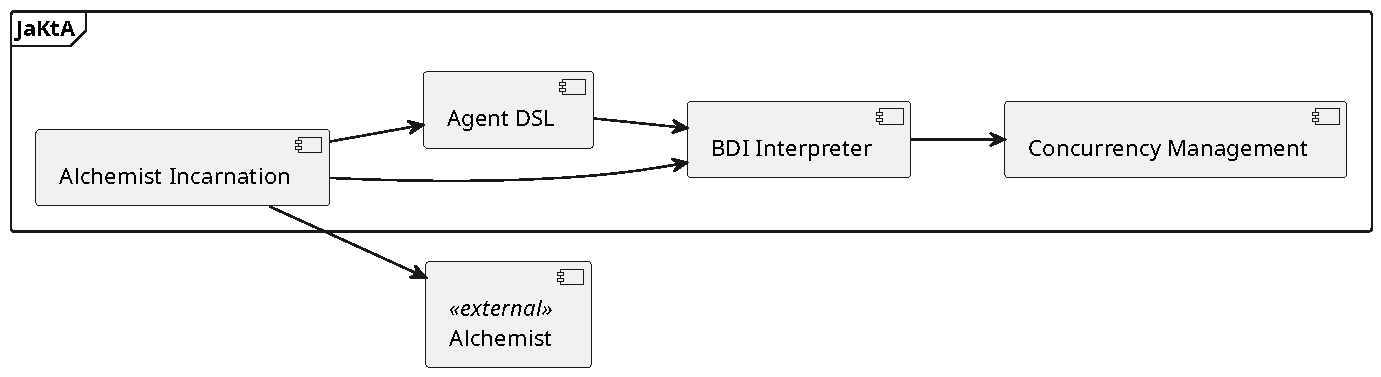
\includegraphics[width=\textwidth]{figures/mas/jakta_modules.pdf}
    \caption{
        The main modules composing the \jakta{} framework and their dependencies.
    }
    \label{fig:jakta-modules}
\end{figure}

The \jakta{} framework is composed of four main modules (\Cref{fig:jakta-modules}), namely:
%
\begin{enumerate}
    \item the \textbf{\ac{BDI} interpreter}, which governs the execution of agents in environments,
    regardless of the particular syntax used to define them;
    \item the \textbf{\ac{DSL}}, which provides a Kotlin syntax to idiomatically define \ac{BDI} \acp{MAS};
    \item the \textbf{concurrency manager}, which regulates runtime, concurrency, and scheduling aspects for
    any system run by the \ac{BDI} interpreter;
    and
    \item the \textbf{\alchemist{} incarnation},
    which bridges the \ac{BDI} interpreter with the \alchemist{}~\cite{PianiniJOS2013} discrete-event simulator.
\end{enumerate}

A detailed description of the \jakta{} syntax is available in \cite{DBLP:journals/sncs/BaiardiBCP24}, for the interested reader.
%
Here some examples of \jakta{} code are reported to showcase the main features of the framework.

\noindent
\begin{minipage}{\linewidth}
\lstinputlisting[
    % float,
    basicstyle=\footnotesize\ttfamily,
    linewidth=\linewidth,
    language=Kotlin,
    caption={Overall structure of a \ac{MAS} specification in \jakta{}.},
    %{Entrypoint of \jakta{}, it contains the description of the Environment and Agents involved in the application.},
    label=lst:mas,
]{listings/jakta-examples/mas_dsl.kt}
\end{minipage}
%
Users can define and launch a \jakta{} \ac{MAS} specification using a \texttt{mas} block (\Cref{lst:mas}).
All elements composing the \ac{MAS} are defined within it, including the (initial) set of agents, the environment model and other \ac{MAS} configuration elements.
%
The \texttt{agent} block in \Cref{lst:mas} defines an individual \ac{BDI} agent,
specifying its initial beliefs and goals, as well as the plan library it will use at runtime.
%
The syntax is valid Kotlin code, which implements at the language level features to support the construction of \acp{DSL} (e.g., lambda with receiver, operator overloading, block-like lambdas, etc.) that can be implemented as \emph{type-safe builders}\footnote{\url{https://kotlinlang.org/docs/type-safe-builders.html}}.
%
This makes the \ac{MAS} specification fully supported by existing Kotlin development tools.

\noindent
\begin{minipage}{\linewidth}
\lstinputlisting[
    % float,
    basicstyle=\scriptsize\ttfamily,
    linewidth=\textwidth,
    language=Kotlin,
    caption={Example of paradigm-blending in \jakta{}. The code snippet uses together \ac{OOP}, \ac{FP}, and \ac{IP} constructs to create a \ac{MAS}.},
    label={lst:blending},
]{listings/jakta-examples/blending.kt}
\end{minipage}
%
% Additionally,
The adoption of a multi-paradigm language such as Kotlin
natively exposes \ac{OOP}, \ac{FP}, and \ac{IP} constructs within the \ac{BDI} \ac{DSL}.
This supports a first level of paradigm blending, which allows composing and parametrizing the \ac{MAS} specification with ease.
%
The blending is exemplified in \Cref{lst:blending},
it describes, using \jakta{} syntax,
a toy example defining a \ac{MAS} with ten agents named as the first ten athletes scraped from a web page.
%
The example showcase the combination of the \ac{OOP} paradigm employed for dealing with regular expressions matching and data extraction,
and the \ac{FP} paradigm used to map URLs to athletes names, and finally to \jakta{} agents.

Further paradigm integration can be leveraged when defining actions.
%
In \jakta{}, a valid action is any instance of the \texttt{Action} interface
(more precisely, of one of its specializations \texttt{InternalAction} or \texttt{ExternalAction}),
and can be written in-place directly inside a \texttt{mas} definition,
possibly using \ac{OOP} or \ac{FP} constructs directly in Kotlin.

\jakta{} has an explicit notion of \emph{environment}. The \jakta{} environment is responsible for:
%
\begin{inlinelist}
    \item tracking the agents in the system;
    \item governing each agent's perception by determining which percepts to deliver;
    \item governing each agent's actuation by making external actions available;
    \item governing communication among agents by deciding how messages are delivered;
    \item enabling stigmergic interaction by making the environment's data accessible to agents.
\end{inlinelist}
%
The basic implementation of the environment acting as a shared data container can be extended to implement more complex functionalities, integrate external systems within the \ac{MAS}, and support distributed communication. 


%=======================================================
\section{Testing \acs{MAS} with Simulation}
\label{sec:mas:engineering:simulation}
%=======================================================

Aside from being useful for in-silico studies,
\emph{simulation} may also aid the \emph{development} and \emph{validation}~\cite{uhrmacher_simulation_2002}
of \acp{MAS} intended for real-world deployment.
%
In fact, simulation enables developers to test the behavior of agents
and their dynamics in complex environments ahead of deployment,
while postponing costs, risks, and efforts associated with real-world execution.

The price for such flexibility, however,
is paid in additional development effort:
first and foremost, to model the deployment context in a simulation environment,
and, additionally,
to maintain alignment between the two versions of the \ac{MAS} codebase,
unless the same \ac{MAS} specification can execute \emph{with no changes}
on both real hardware and a simulator of choice.

This is particularly challenging when dealing with \ac{BDI} \acp{MAS}.
There,
the abstraction gap between the high-level cognitive model of \ac{BDI} agents and most simulators~\cite{singh_integrating_2016},
along with the minimal support of \ac{BDI} technologies
for producing \emph{reproducible} simulations of articulated scenarios~\cite{kehoe2016robust}
lead developers to resort to one of the following approaches~\cite{singh_integrating_2016}:
%
\begin{enumerate}
    \item extension of the \ac{BDI} platform with a dedicated simulation engine,
    which requires additional development effort (e.g., \cite{HubnerB09,ricci_exploiting_2020});
    \item construction and maintenance of two parallel codebases
    one for a simulator extended with \ac{BDI} modeling tools (e.g., \cite{sakellariou_enhancing_2008,TaillandierBCAG16,uhrmacher1998agents}) and one for the actual system,
    leading to consistency issues;
    \item integration of the \ac{BDI} platform with a general-purpose simulation engine,
    typically by synchronizing their execution through some form of middleware (e.g., \cite{singh_integrating_2016,davoust_architecture_2020}).
\end{enumerate}

Despite the idea of using simulation to support \ac{MAS} development being not new
there are not many tools that effectively allow one
\emph{
    ``to execute agents as they are and to switch arbitrarily between execution in the real environment and the virtual test environment''
}~\cite{uhrmacher_simulation_2002}.

This section discusses the challenges of decoupling \ac{BDI} agent concurrency when designing \ac{MAS} frameworks, as a necessary step towards enabling the same specification to run both in real concurrent deployments and in discrete-event simulation environments.
%
The proposed integration of \jakta{} with the \alchemist{} simulator explores the mapping of the \ac{BDI} control loop, showing that different granularities are possible, to address the challenge of providing a seamless transition between real and simulated environments for \ac{BDI} \acp{MAS}.

%-------------------------------------------------------
\subsection{Decoupling Concurrency in BDI MAS}
\label{ssec:mas:engineering:concurrency}
%-------------------------------------------------------

The analysis of a selection of technologies from table \Cref{tab:frameworks} presented in \cite{DBLP:conf/emas/BaiardiBCPRO24} suggests that most \ac{BDI} frameworks tightly couple the \ac{BDI} control loop with the underlying \emph{concurrency model}. 
%
This means that the way in which agents are scheduled and executed is often hardcoded into the framework, limiting flexibility and adaptability to different application requirements.

Several concurrency models are possible for \ac{BDI} \ac{MAS}: 
\begin{itemize}
    \item \emph{\ac{1A1T}}: is the most common where each agent runs in a dedicated thread. This model provides true parallelism but can lead to high resource consumption. 
    \item \emph{\ac{AA1T}}: the degenerate case where all agents run in a single thread, leading to sequential execution (e.g. round-robin scheduling), agents do not run in parallel, but the system is lightweight and easier to debug.
    \item \emph{\ac{AA1EL}}: at the conceptual level is similar to \ac{AA1T}, but instead of using threads, it employs an event loop to manage agent execution. This model is efficient and suitable for handling blocking operations in the agent logic.
    \item \emph{\ac{AA1E}}: similarly to \ac{AA1EL} but there is a shared executor allowing for concurrent execution of agents while still benefiting from the efficiency of event-driven programming. Scaling the executor allows for tuning the level of resource usage and parallelism.
\end{itemize}

Decoupling the specification of the adopted concurrency model from the \ac{BDI} control loop allows to select the most appropriate model for different applications.
%
This requires defining clear interfaces between the \ac{BDI} interpreter and the concurrency manager when designing \ac{BDI} frameworks.
%
Each agent control-loop phase (e.g., perception, deliberation, action) should be treated as a task that can be scheduled on a concurrency abstraction.
%
This decoupling can also serve the purpose of switching between real and simulated execution, as the simulator would act as yet another \emph{executor} of \ac{BDI} tasks.

%-------------------------------------------------------
\subsection{Discrete-Event Simulation for BDI}
%-------------------------------------------------------

\ac{DES} is a powerful technique for modeling complex systems, that can support the scheduling of events over simulated time, and advance the simulation clock to when the next event is due.
%
Given the fact that \ac{BDI} agents can be seen as driven by events (e.g., percepts, messages, internal triggers), \ac{DES} appears as a natural fit for simulating \ac{BDI} \acp{MAS}. 
%
\ac{DES} allows for a fine-grained control over the timing and ordering of events, making it possible to accurately model the asynchronous and concurrent nature of agent interactions.

The integration of a \ac{BDI} \ac{MAS} over a \ac{DES} simulator require mapping the \ac{BDI} control loop iterations onto the simulator's event scheduling.
%
Different granularities of mapping are possible, each with its own trade-offs:
\begin{itemize}
\item \emph{\ac{AMA}}: the entire \ac{MAS} advances in lockstep, with all agents performing one iteration of the control loop in a sequential order at every step. This is the coarsest granularity, usually adopted when simulating \ac{BDI} agents for debugging purposes (e.g., \cite{HubnerB09}).
\item \emph{\ac{ACLI}}: each full iteration of the agent's control loop is treated as a single event. Interleave of agent actions is possible, but the agent execution is treated as atomic steps and cannot model the duration of individual phases.
\item \emph{\ac{ACLP}}: each phase of the control loop (perception, deliberation, action) is mapped to separate events. This allows for more detailed modeling of agent behavior and interactions. All possible interleaving are possible, like in a true concurrent system and hence providing the most accurate simulation of real-world execution.
\item \emph{\ac{ABE}}: each event in the \ac{BDI} agent (e.g., perception, message receipt, internal trigger) is mapped to a discrete event in the simulator. This allows for fine-grained simulation but may increase the number of scheduled events significantly, potentially impacting performance of the simulation, while not providing significant benefits over \ac{ACLP} in most scenarios as the behavior of agents encapsulate its internal events.
\end{itemize}

Other than choosing the appropriate granularity for the mapping, switching between real and simulated execution requires careful handling of time management and \emph{external actions} that are invoked on the environment.

In real execution, time can be perceived from the system clock, while in simulation, time is controlled by the simulator.
%
Therefore, agents must be designed to use a time abstraction that can be adapted to both real and simulated contexts.
%
The same goes for randomness, which should be abstracted to allow for reproducible simulations controlled by the same \emph{seed}. 

For what concerns environment actions, modeling the environment is crucial for accurate simulation. 
%
The agent should be decoupled by the specific implementation of the environment, relying on an interface that can be implemented differently for real and simulated contexts.
%
The simulated environment should mimic the behavior of the real environment as closely as possible, including the generation of perceptions, the effects of actions that modify the environment state and the communication mechanisms among agents which may need to be tested for reliability under different conditions. 

The design of \jakta{} has been influenced by these considerations.
%
This made it possible to integrate \jakta{} with the \alchemist{} \ac{DES} simulator~\cite{PianiniJOS2013}.
%
The integration is achieved by letting \alchemist{} schedule the execution of \jakta{} agents by scheduling their control loop iterations and phases with a time distribution.
%


%-------------------------------------------------------
\subsection{Experimental Demonstrator}
%-------------------------------------------------------

The prototype implementation demonstrates the feasibility of the approach, and showcases how different granularities of mapping can lead to different simulation behaviors with the same \ac{MAS} specification.

To exemplify this, a simple \ac{MAS} is defined to simulate a leader \ac{UAV} moving in a circular path, while other \acp{UAV}
must follow its movement retaining their formation around the leader.

\Cref{fig:code} shows code extracts from the scenario implementation, demonstrating that agent logic is reusable across different execution platforms.

\begin{figure}
    \begin{minipage}[b]{.6\linewidth}
        \centering
        \lstinputlisting[
            language=Kotlin,
            linewidth=\linewidth,
            basicstyle=\scriptsize\ttfamily,
            label={lst:logic},
    %        caption={Platform-agnostic code}
        ]{listings/jakta+alchemist/agentsLogic.kt}
    \end{minipage}
    \hfill
    \begin{minipage}[b]{.34\linewidth}
        \centering
        \lstinputlisting[
            language=Kotlin,
            linewidth=\linewidth,
            basicstyle=\scriptsize\ttfamily,
%        caption={Entrypoint},
            label={lst:agents}
        ]{listings/jakta+alchemist/agents.kt}
    \end{minipage}
    \caption{
        The agent specifications (left) are completely platform-agnostic and reusable,
        some glue code (right) wires the logics with the underlying execution platform.
    }
    \label{fig:code}
\end{figure}


To investigate the effect of the mapping granularity on the system's behavior, experiments are conducted with the \ac{AMA}, \ac{ACLI}, and \ac{ACLP} granularities.
%
To do so, \ac{AMA} is used as baseline,
letting the entire \ac{MAS} run a full cycle every simulated second.
%
Then the baseline is compared with \ac{ACLI} and \ac{ACLP},
for which each agent is modeled with an execution frequency $f$
following a Weibull distribution with mean $f$ and deviation $f\cdot\tau$ modeling the \emph{relative drift} in the internal clock of different devices.
%
Additionally, for the \ac{ACLP} granularity deliberation and action delays are modeled,
associating each phase with an exponential distribution with rate $\lambda = f$:
faster agents (larger $f$ values) have less delay.
%
Every experiment is repeated $100$ times with a different random seed, changing
the initial positions of the followers
and the distribution in time of the events for the \ac{ACLI} and \ac{ACLP}.

\begin{figure}
    \centering
    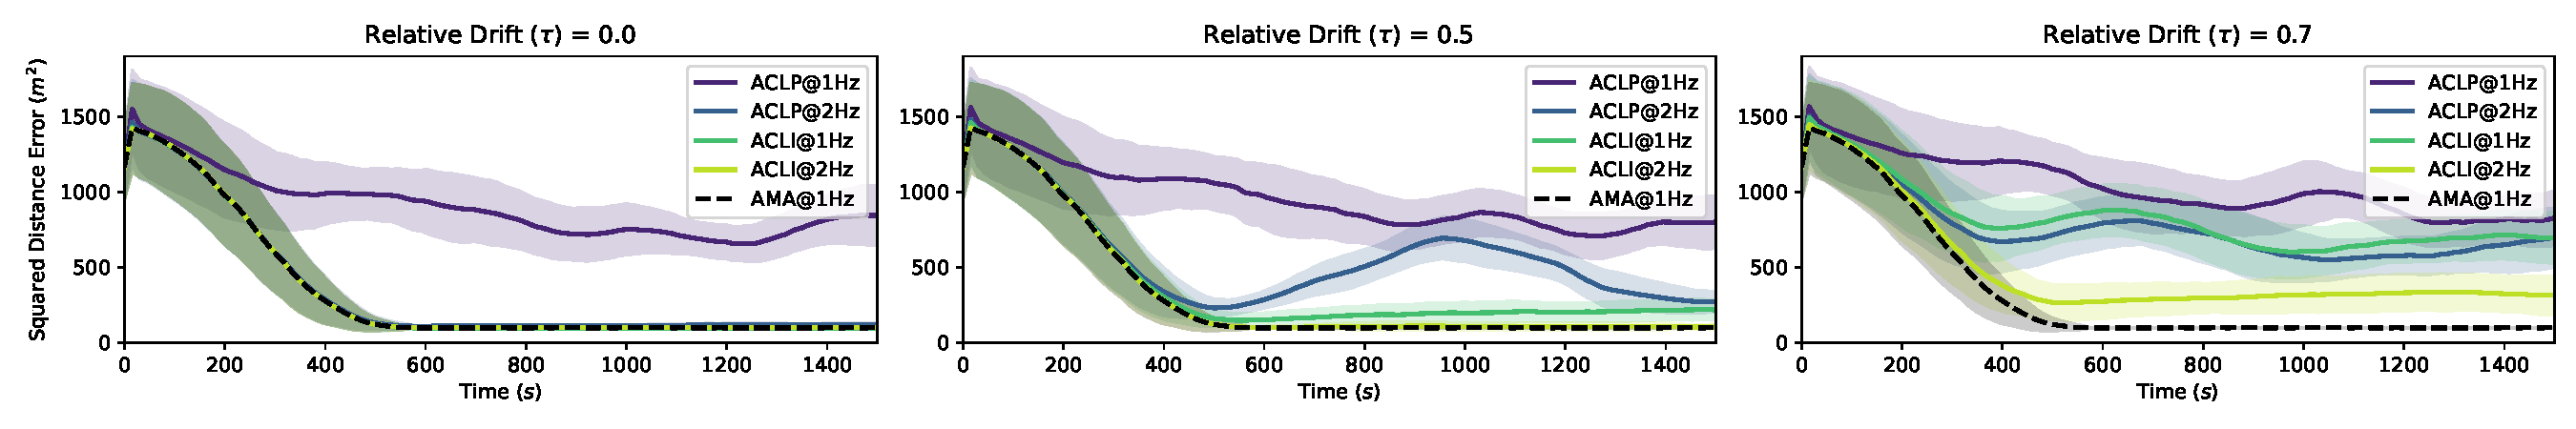
\includegraphics[width=\linewidth]{figures/jakta+alchemist/error_over_time_flattened.pdf}
    \caption{
        Average error with time for different granularities, with \ac{ACLI} and \ac{ACLP} running at $f=1Hz$ and $f=2Hz$.
        Different charts show different values of relative drift $\tau$.
        Coloured shadows represent $\pm 1\sigma$ over multiple runs.
    }
    \label{subfig:err_time}
\end{figure}
%
% \begin{figure}
%     \centering
%     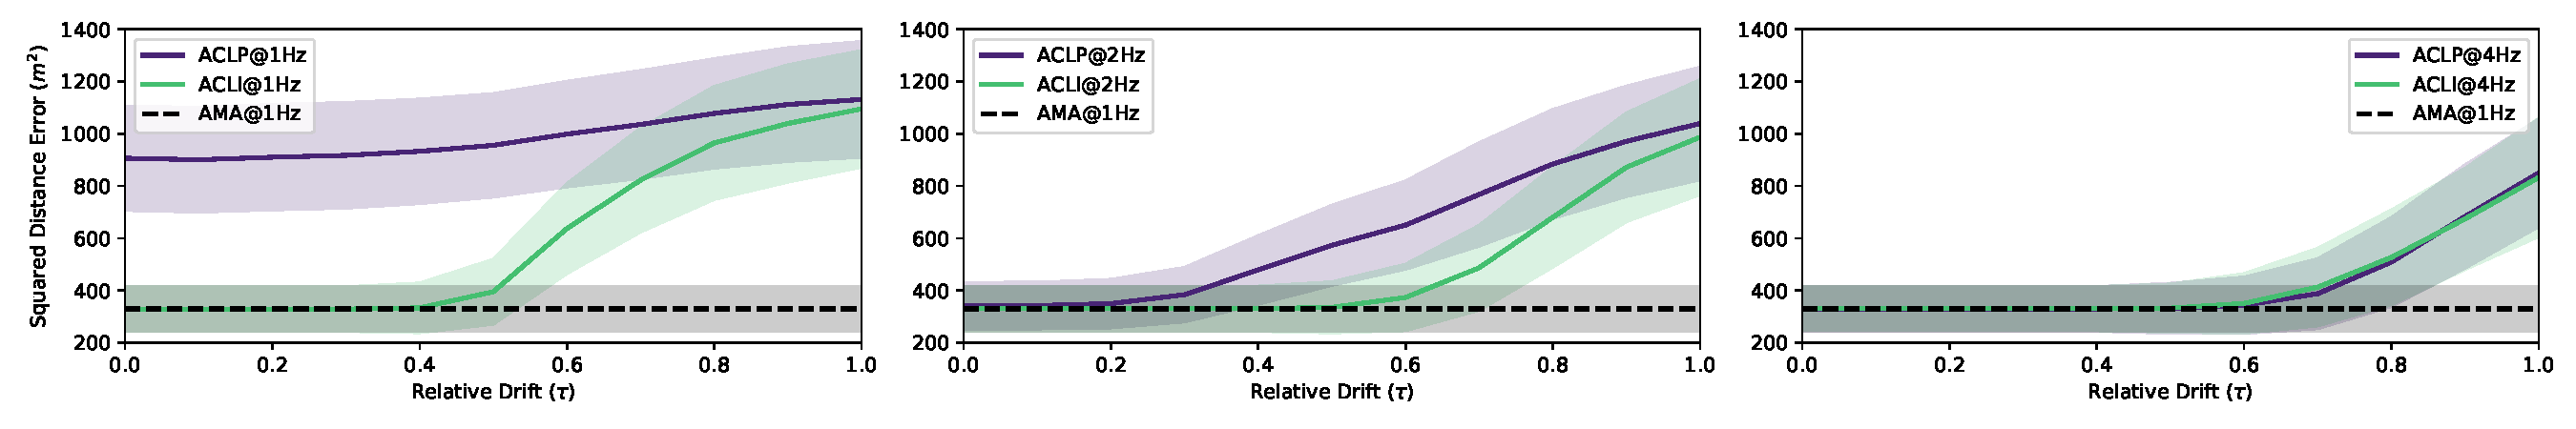
\includegraphics[width=\linewidth]{figures/jakta+alchemist/error_over_variances.pdf}
%     \caption{
%         Mean squared distance error with relative drift ($\tau$), measured for different frequencies for \ac{ACLI} and \ac{ACLP}.
%         Coloured shadows represent $\pm 1\sigma$.
%     }
%     \label{subfig:err_drift}
% \end{figure}
\Cref{subfig:err_time} shows the error on the followers position with respect to the ideal formation over time as the mean square distance of all followers \acp{UAV}.
As expected given the simplistic implementation of the agent's logic, the \ac{AMA} granularity appears to be the most stable, converging quickly to a low error.
%
Differently from \ac{AMA}, both \ac{ACLI} and \ac{ACLP} instead, show a degradation in performance at low frequencies and higher relative drifts.
%
This is due to the fact that the implementation assumed implicit synchronization among agents and virtually no-delay in the perception-action loop (which is the case in \ac{AMA}), but fail to adapt fast enough when the execution is asynchronous and delayed, similarly to real-world deployments.

This showcase demonstrates that selecting fine-grained granularities for mapping the \ac{BDI} control loop into \ac{DES} events is necessary to accurately simulate real-world deployments, thus supporting the argument that the \ac{BDI} framework should expose the ability to finely decouple the execution of individual phases of the control loop from the concurrency model.

%=======================================================
\section{BDI Agents in Hypermedia Environments}
%=======================================================

As discussed in \Cref{sec:back:mas:web}, the Web is increasingly being seen as a \emph{hypermedia environment} where autonomous agents can operate and interact with resources through \ac{REST} interactions, and by consuming semantic descriptions of resources and services.

Even more recently,
with the advent of \ac{LLM}-based \emph{Agentic AI}~\cite{Acharya_Kuppan_Divya_2025}
the creation of \ac{LLM}-driven agents that interact with Web APIs~\cite{10.5555/3692070.3692540}
(or directly with Websites~\cite{10.5555/3692070.3694608})
has gained significant attention.
%
However,
despite being promising,
these approaches
do not make structured knowledge representation obsolete~\cite{pan2024tkde},
and often trade the controllability offered by traditional agent-programming paradigms
for more guarantees in terms of correctness, and completeness.

Arguably,
Web-integrated agents developed with cognitive architectures,
such as \ac{BDI} agents,
would retain controllability and predictability:
they could directly exploit hypermedia to discover new resources and actions,
and use Semantic Web technologies like \ac{RDF} and \ac{OWL}
to act intelligently without compromising on quality.
%
However,
it can be argued that
the integration of \ac{BDI} agents with the Web
is hindered by a conceptual and technological gap,
which limits developers in creating agents that need to interact with (Semantic) hypermedia.
%
More precisely:
\begin{itemize}
  \item\label{gap:logic}
  \ac{BDI} agents are historically tied to \ac{LP}
  %-- e.g., with the popular \agentspeak{} semantic~\cite{DBLP:conf/maamaw/Rao96} --
  whereas the Semantic Web is grounded on description logic,
  and although the two paradigms are theoretically compatible,
  their practical implementations interoperate poorly,
  increasing integration cost significantly;
  % The different technological choices used to concretely implement them add cognitive load to developers working on the integration of the two worlds (e.g., converting \ac{OWL} and \ac{RDF} triples in Prolog-like formulas);

  \item\label{gap:open-world}
  \ac{BDI} agents are typically based on the \ac{PRS} architecture~\cite{georgeff1987reactive}
  which relies on pre-defined plans and does not natively support discovering new actions at runtime,
  a necessary feature to interact proficiently with hypermedia environments.
\end{itemize}

In \cite{burattini2025gap}, a detailed analysis of these gap is presented, reflecting on the nuances of different models and concrete syntaxes used for logic representation, query semantics and inference mechanisms.
%
The analysis results in the definition of a set of requirements that can guide future research on bridging the gap between \ac{BDI} agents and hypermedia environments.
%
For a deeper integration of \ac{BDI} agents with semantic hypermedia environments, the following requirements should be addressed:
\begin{enumerate}[label=\textbf{(R\arabic*)}]
  \item direct manipulation of \ac{RDF} and \ac{OWL} triples in the agent's belief base;
  \label{req:direct}

  \item ontological inference for deliberation (e.g., plan selection and execution);
  \label{req:reasoning}

  \item support for querying the belief base via \acs{SPARQL};
  \label{req:query}

  \item ability to exploit affordances discovered in the environment to dynamically adapt the agents' plans.
  \label{req:actions}
\end{enumerate}

%--------------------------------------------------------------
\subsection{A Generalized BDI Engine}
%--------------------------------------------------------------

Towards addressing \ref{req:direct}, \ref{req:reasoning}, and \ref{req:query}, \cite{burattini2025gap} proposed the development of a generalized \ac{BDI} engine that can be specialized to work with different belief, goal, plan representations and reasoning mechanisms. 
%
A similar approach has been proposed in~\cite{novak2006atal}, 
in which authors discuss the idea of a modular \ac{BDI} architecture,
to make it independent of the logic representation and reasoning mechanisms,
although not in the context of hypermedia.
%
Sharing the core modularity idea, the proposal of a generalized \ac{BDI} interpreter encapsulating agents reasoning cycle,
while decoupling the specific technology used for knowledge representation and manipulation would allow for tailoring the reasoning mechanisms to application-specific needs.
%
In this way,
beliefs
can flexibly support different formats depending on the domain at hand
and be adapted to work directly with e.g., \ac{RDF} triples, to JSON, YAML, and other Web standards.

Similarly, the fundamental operations performed by a \ac{BDI} agent (e.g., plan selection, belief update, goal adoption), could be implemented using customized mechanisms that leverage the specific semantics of the adopted representation.

\begin{figure}
    \centering
    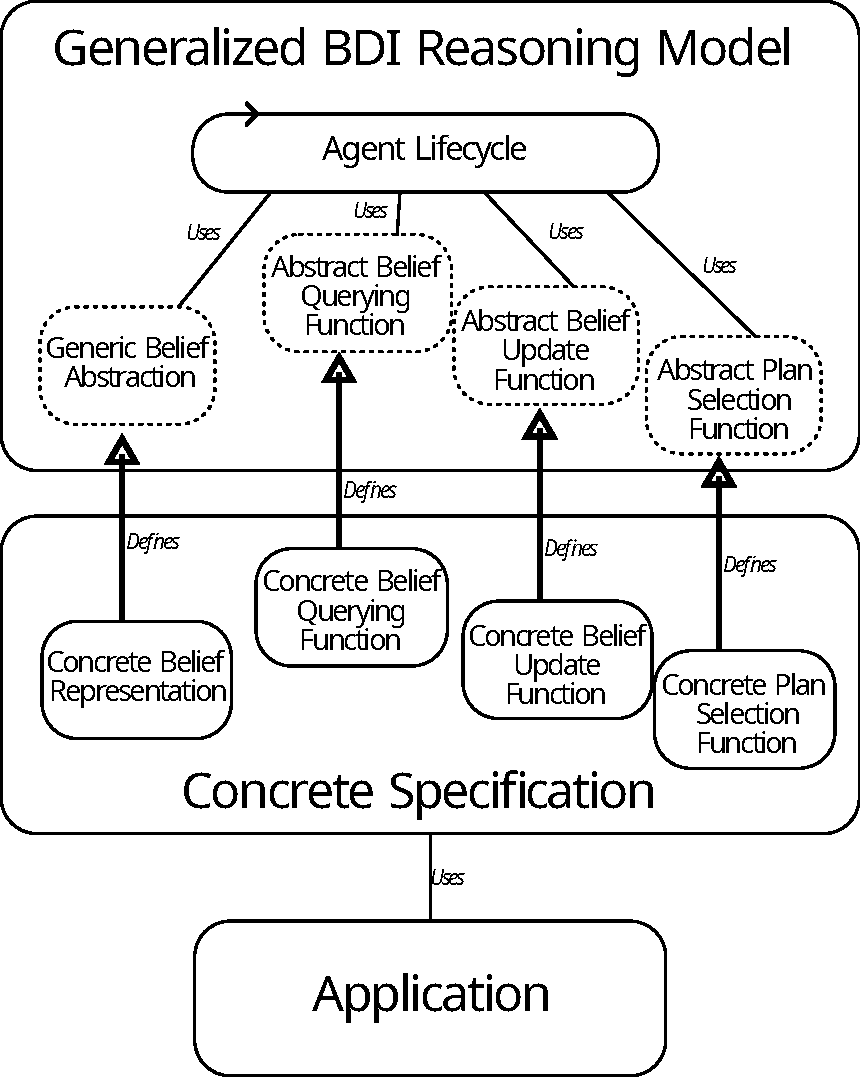
\includegraphics[width=0.8\textwidth]{figures/generalize_bdi.pdf}
    \caption{
        The generalized \ac{BDI} engine architecture.
        The core \ac{BDI} reasoning cycle is decoupled from the specific implementations of beliefs, goals, plans, and reasoning mechanisms.
        This allows for specializing the engine to work with different representations and logics.
    }
    \label{fig:generalized-bdi-engine}
\end{figure}


\Cref{fig:generalized-bdi-engine} schematically illustrates the architecture of the proposed \ac{BDI} engine showing three layers:
\begin{itemize}
  \item \textbf{generalized \ac{BDI} reasoning layer},
  where the agent's deliberation process is implemented as a reasoning cycle,
  yet agnostic to how beliefs are represented and manipulated.
  %
  This is where
  agents' intentions are maintained
  and updated as agents perceive,
  decide what to do,
  and finally act.
  %
  Any operation involving beliefs, or plan selection, should rely on some \emph{abstract} \acs{API},
  to be implemented by the next layer.
  %
  \item \textbf{concrete specification layer},
  where the aforementioned \acs{API} is implemented to provide concrete operations on the belief base and plan library.
  %
  This layer acts as an adapter between the generalized \ac{BDI} reasoner
  and the specific knowledge representation technologies of choice.
  %
  Lastly,
    \item \textbf{application layer},
  where actual goals, plans, and interactions of a \ac{MAS} are defined
  to tackle some specific use case.
\end{itemize}

This architectural blueprint is a starting point, to which the \jakta{} framework (\Cref{sec:mas:engineering:jakta}) is intended to evolve, to better support the integration of \ac{BDI} agents with other kinds of systems, including hypermedia environments. 

%-------------------------------------------------------
\subsection{Embodiment for Agents on the Web}
%-------------------------------------------------------

When considering open, dynamic, and large-scale systems where different agents may join and leave a shared environment at any time, the ability to \emph{discover information about other agents} becomes a crucial factor for enabling interaction.
%
One way to enable the discovery of agents in such open systems is to equip them with \emph{bodies} that are reified in the shared environment.
Such bodies may also permit agents to communicate indirectly through reciprocal observation of their actions, facilitate contextual interaction, and support accountability mechanisms through the observability of visible agent behavior---all of which is enabled through embodiment.
%
The body itself becomes an indicator of an agent's presence, offering means to perceive its (observable) state and actions---and possibly even to ascribe goals to the agent~\cite{castelfranchi2012abscribingminds}.

Software agents are typically defined as \emph{situated} (\Cref{chap:back:MAS}), but not necessarily \emph{embodied} as the two properties are not dependent on each other when considering virtual environments.
%
On the Web, being \emph{situated} implies agents can browse the Web by discovering and following links from page to page. However, the agents are not \emph{embodied}: Multiple agents browsing the same website are typically unaware of one other, as there is no representation of the other agents currently \emph{on} the same page.
%
This does not preclude \textit{designing} websites that support embodiment---and this can be witnessed regularly, for instance, in collaborative document editors. However, such support must be designed and implemented explicitly into the website.

Following the proposal of \ac{hMAS} to make all significant entities in a \ac{MAS} represented within the hypermedia environment~\cite{Ciortea_Boissier_Ricci_2019}, it is possible to design an agent body as a Web resource that other agents can discover and interact with. 
%
A step in this direction is taken in~\cite{Zimmermann2023}, which motivates the need for agents' situatedness and embodiment in open hypermedia environments and illustrates a potential solution based on the Solid specifications~\cite{Solid_0.9.0:21}. The authors outline several requirements for agent embodiment in decentralized hypermedia systems, but they do not provide a conceptual model for agent bodies as first-class abstractions which can guide the design of digital embodiment in \ac{hMAS} and other kinds of virtual environments.

\cartago{} (\Cref{sec:back:mas:aose}) which is an inspiration for \ac{hMAS} provides an implementation of agent bodies as \emph{artifacts} that are automatically assigned to agents when they join a \emph{workspace}~\cite{Ricci_Piunti_Viroli_Omicini_2009}.
%
The artifact serves as a proxy to the agent in the shared environment, enabling \cartago{} to support heterogeneous agents in the same environment.

Following these ideas, \cite{embodiment2025} proposes a conceptual notion of \emph{agent body} for \ac{hMAS} based on the following set of features:
\begin{itemize}
    \item \textbf{Discoverability}: bodies should enable agents to discover one another in an environment and optionally identify the corresponding agent associated to it. 
    \item \textbf{Communication Through Behavior}: bodies should enable implicit communication between agents through their observable behavior, by showing the actions being performed by the agent.
    \item \textbf{Accountability}: bodies should support accountability mechanisms by making the agent's actions and state observable.
    \item \textbf{Situation-Dependent Interaction}: bodies should facilitate interaction by exposing contextually relevant information about the agent as well as affordances to interact with it.
\end{itemize}

To support such desired features, the agent body is hence defined as:
\begin{quotation}
A body is an artifact reifying and identifying an agent in an environment. The body situates the agent, transparently mediating its actions and allowing the agent to perceive in a timely fashion.
The body allows others to observe the owner agent and its behavior, and to perceive agent-specific affordances to interact with it.
\end{quotation}

This definition captures the fundamental properties of an agent body in virtual environments, emphasizing its role in reifying the agent (\textbf{concreteness}), identifying it (\textbf{identifiability}), implicitly mediate actions (\textbf{transparency}), routing perceptions from the environment (\textbf{timely perception}) and allowing other agents to observe the agent's behavior through it (\textbf{focusability})~\cite{embodiment2025}.

\begin{code}
\captionof{listing}{A description of agent {\tt alice} and its body artifact.}
\label{lst:agent-description}
\begin{minted}{turtle}
@base <http://localhost:8080/> .
@prefix hmas: <https://purl.org/hmas/> .
@prefix td: <https://www.w3.org/2019/wot/td#> .
@prefix jacamo: <https://purl.org/hmas/jacamo/> .

<workspaces/production/artifacts/alice/#artifact> a td:Thing, hmas:Artifact, jacamo:Body;
  hmas:isContainedIn <workspaces/production/#workspace>;
  jacamo:isBodyOf <workspaces/production/agents/alice/#agent>;
  td:hasActionAffordance [ a td:ActionAffordance, jacamo:Focus;
    td:name "focus";
    td:hasForm [ htv:methodName "POST";
      hctl:hasTarget <workspaces/production/artifacts/alice/focus>;
      hctl:forContentType "application/json";
      hctl:hasOperationType td:invokeAction ];
    td:hasInputSchema [ a js:ObjectSchema;
      js:properties [ a js:StringSchema;
        js:propertyName "callbackURI"]
    ]].

<workspaces/production/artifacts/alice/#agent> a hmas:Agent .
<workspaces/production/#workspace> a hmas:Workspace .
\end{minted}
\end{code}

\Cref{lst:agent-description} shows an example of implementation of an agent body as an artifact within an hypermedia environment exposed by the Yggdrasil platform~\cite{Ciortea_Boissier_Ricci_2019}.
%
Through \ac{RDF} triples, the agent \texttt{alice} is described as an instance of \texttt{hmas:Agent} (with the \ac{hMAS} ontology~\cite{hmas-core}), and its body is shown as currently contained in a workspace, situating the agent in the hypermedia environment.
%
The body artifact is also identified as an instance of \ac{WoT} \emph{Thing}~\cite{wot-td}, and exposes an action affordance \texttt{focus} that other agents can invoke to observe \texttt{alice}'s body (e.g., to monitor its behavior).

The definition of agent bodies for \ac{hMAS} opens up interesting research directions towards better supporting societies of agents operating in hypermedia environments. 
%
\ref{req:actions} assumes particular importance in this context, as agents would not only discover actions exposed by passive \emph{artifacts} in the environment, but possibly also from other agents through their bodies. 

%-------------------------------------------------------
\subsection{Enhancing BDI Agent Adaptability}
%-------------------------------------------------------

This section briefly reports contributions in the area of enhancing the adaptability of \ac{BDI} agents towards addressing \ref{req:actions}.
%
Although not directly focused on hypermedia environments, the proposed approaches can be extended to such contexts to improve agent adaptability in open and dynamic environments.
This follows the ideas presented in Section~5.4 of \cite{Boissier_Ciortea_Harth_Ricci_Vachtsevanou_2023}, which discusses the enhancement of agents through a set of reusable strategies that can support their exploration of open environments such as the Web.

Along this line of research,
\cite{Ciatto_Aguzzi_Battistini_Baiardi_Burattini_Ricci_2025} proposes an approach to leverage the generative capabilities of \acp{LLM} to generate plans on-the-fly, based on the current context and goals of the agent.
%
Although still in preliminary stages, this approach can significantly enhance the adaptability of \ac{BDI} agents in dynamic environments, as they can generate new plans when existing ones are not suitable for the current situation.
%
In hypermedia environments, where agents might be programmed to expect specific structures or resources, the ability to generate plans dynamically can help them adapt to unexpected changes.
%
\ac{LLM} can also be used to interpret the semantics of Web resources and map relevant information to the agent's beliefs and goals, possibly guiding the adaptation process.
%
The exploitation of \ac{GenAI} techniques for the design of agents is an open research direction, to which \ac{BDI} agents can contribute by providing a structured framework of cognitive abstractions that support the design and interpretation of autonomous behavior~\cite{DBLP:conf/atal/Ricci0ZBC24}.


A different approach is taken in \cite{DBLP:journals/aamas/HubnerBRM25}, 
where a proposal for enabling \ac{BDI} agents to forecast their behavior in a simulated environment before acting in the real deployment context is presented as a way to detect future issues and adapt accordingly by refining ordering of options.
%
\cite{wesaac} further explores this idea when considering multiple future-oriented \ac{BDI} agents, noticing how, without the exchange of information, agents may still end up in conflicting situations as they adapt their behavior based on their individual forecasts which may miss the effects of other agents' actions.

This approach can be particularly useful in hypermedia environments,
where the dynamics of the environment and the presence of other agents can lead to unexpected situations.
%
In this context, \acp{DT} can actually help agents to simulate their actions in a controlled environment, letting agents play out their plans on a simulation of the \ac{PA} first to detect potential issues and react accordingly.
%
This opens up interesting future research directions on the interplay of adaptable \ac{BDI} agents and \acp{DTE}~\cite{DBLP:conf/eumas/Burattini23}.


%=======================================================
\section{Explainability in \acs{BDI} Agents}
%=======================================================

%-------------------------------------------------------
\subsection{Multi-Level Explainability}
%-------------------------------------------------------


%-------------------------------------------------------
\subsection{Inter-Agent Explainability}
%-------------------------------------------------------


%=======================================================
\section{Final Remarks}
%=======================================================

